\documentclass[20pt]{article}
\usepackage[utf8]{inputenc}
\usepackage{amsmath, amssymb, amsthm}
\usepackage{titlesec}
\usepackage{pgfplots}
\usepackage{graphicx}
% Customization -------

% Paper size, margin
\usepackage[letterpaper,top=1.5cm,bottom=1.5cm,left=1.75cm,right=1.75cm,heightrounded]{geometry}

% line height
\renewcommand{\baselinestretch}{1.15} % line space

% Paragraph indentation 
\setlength{\parindent}{0pt} % no indent

% Paragraph spacing
\setlength{\parskip}{0.8em} % space between paragraphs

% Section number formatting
\titleformat{\section}[hang]{\bfseries}{Problem \thesection\ }{0pt}{}


% Equation numbering per section
\counterwithin*{equation}{section}
\counterwithin*{equation}{subsection}

% Graphics path
\graphicspath{ {./images/} }

% --------------------

\title{ECE421: Assignment 03}
\author{Farbod Mohammadzadeh\\
    1008360462}
\date{11 October 2023}

\begin{document}
\Large


\maketitle

\newpage

\section{}

\subsection*{\underline{Part 1:}}
Points:
\begin{eqnarray}
    x^{(1)} =  \begin{bmatrix}
        1 \\
        1
    \end{bmatrix},
    x^{(2)} = \begin{bmatrix}
        -1 \\
        -1
    \end{bmatrix},
    x^{(3)} = \begin{bmatrix}
        1 \\
        0
    \end{bmatrix},
    x^{(4)} = \begin{bmatrix}
        0 \\
        1
    \end{bmatrix} \\
    t^{(1)} = 1, t^{(2)} = -1, t^{(3)} = -1, t^{(4)} = -1
\end{eqnarray}
Graph:
\begin{figure}[h]
    \centering
    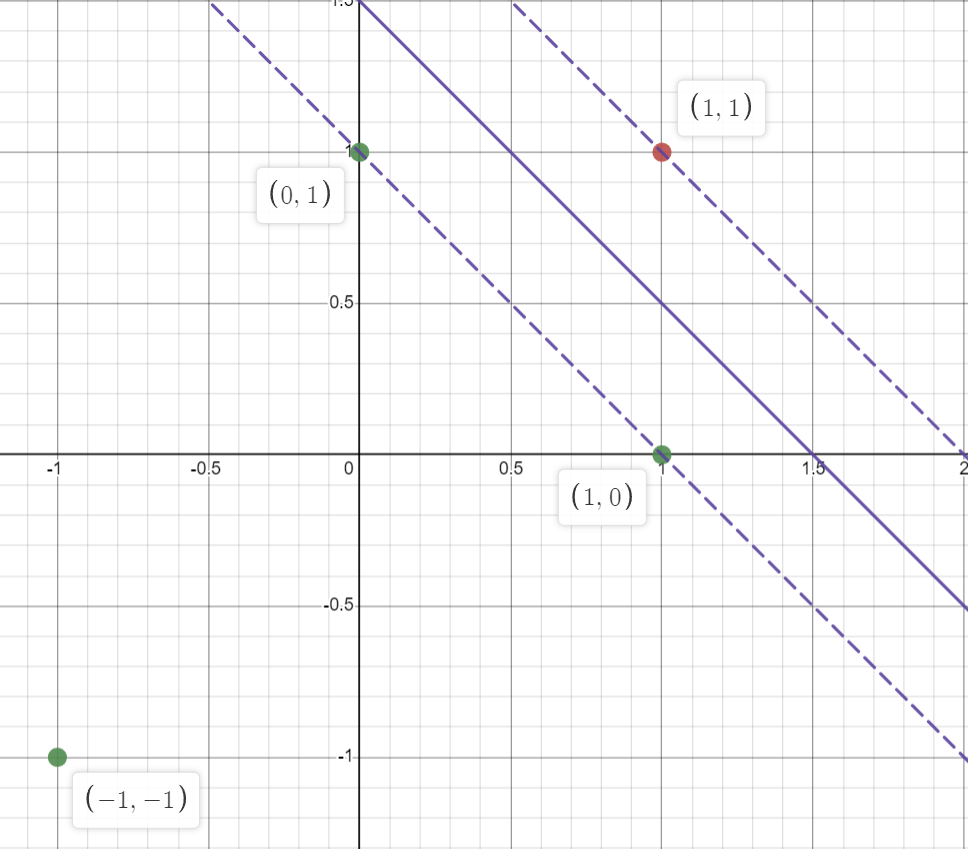
\includegraphics[width=10cm]{desmos-graph}
    \caption{Plot of the points}
    \label{fig:points}
\end{figure}
The equation for the decision boundary is: $y\ =\ -x+1.5$. And the equation for the margins are: $y\ =\ -x+1.5 \pm0.5$.

\newpage

\subsection*{\underline{Part 2:}}
From the above figure \ref{fig:points}, we can see that the support vectors are $x^{(1)}$, $x^{(3)}$, and $x^{(4)}$.
\newpage

\subsection*{\underline{Part 3:}}
We have $\text{argmin}_{\omega,b} \frac{1}{2}\left\lVert \omega \right\rVert^2$ while the constraint of $t^{(n)}(\omega^Tx^{(n)}+b) \geq 1 \ \forall n$ holds over the support vectors. We can rewrite this as the following Lagrangian:
\begin{equation}
    \label{eqn:Lagrangian}
    \mathcal{L} (\omega,b,\alpha) = \frac{1}{2}\left\lVert \omega \right\rVert^2 - \sum_{n=1}^{N} \alpha_n \left( t^{(n)}(\omega^Tx^{(n)}+b) - 1 \right)
\end{equation}
Where each $\alpha_n$ is the Lagrange multiplier for the $n$th data point. We can then take the partial derivatives of $\mathcal{L}$ with respect to $\omega$ and $b$ and set them to zero to find the optimal $\omega$ and $b$.
\newpage

\subsection*{\underline{Part 4:}}
To solve the inner minimization problem, we can first take the partial derivative of $\mathcal{L}$ with respect to $\omega$ and set it to zero:
\begin{align}
    \frac{\partial \mathcal{L}}{\partial \omega} & = \frac{\partial}{\partial \omega} (\frac{1}{2}\left\lVert \omega \right\rVert^2 - \sum_{n=1}^{N} \alpha_n \left( t^{(n)}(\omega^Tx^{(n)}+b) - 1 \right)) = 0
    \\ & = \omega - \sum_{n=1}^{N} \alpha_n (\omega^T x^{(n)} t^{(n)} + b t^{(n)} -1) = 0
    \\ & = \omega - \sum_{n=1}^{N} \alpha_n t^{(n)}x^{(n)} = 0
    \\ \therefore \omega & = \sum_{n=1}^{N} \alpha_n t^{(n)}x^{(n)}
\end{align}
Additionally, we can take the partial derivative of $\mathcal{L}$ with respect to $b$ and set it to zero:
\begin{align}
    \frac{\partial \mathcal{L}}{\partial b} & = \frac{\partial}{\partial b} (\frac{1}{2}\left\lVert \omega \right\rVert^2 - \sum_{n=1}^{N} \alpha_n \left( t^{(n)}(\omega^Tx^{(n)}+b) - 1 \right)) = 0
    \\ & = - \sum_{n=1}^{N} \alpha_n t^{(n)} = 0
    \\ \therefore \ 0 & = \sum_{n=1}^{N} \alpha_n t^{(n)}
\end{align}
From these results we can reorganize the relational equations as:
\begin{equation}
    A = \sum_{n=1}^{N} B_n C^{(n)}D^{(n)}
    , G = \sum_{n=1}^{N} E_n F^{(n)}
\end{equation}
Such that:
\begin{equation}
    A = \omega
    , B_n = \alpha_n
    , C^{(n)} = t^{(n)}
    , D^{(n)} = x^{(n)}
    , E_n = \alpha_n
    , F^{(n)} = t^{(n)}
    , G = 0
\end{equation}


\end{document}